%! Author = Carl
%! Date = 2024/3/3

% Preamble
\documentclass[11pt]{article}

% Packages
\usepackage[T1]{fontenc}% optional T1 font encoding
\usepackage{graphicx}
\usepackage{color}
\usepackage{cite}
%\usepackage{tgpagella}
\usepackage{libertine}
\usepackage{subfigure}
\usepackage{amsmath}
\usepackage{amsthm}
\usepackage{ctex}
\usepackage{geometry}
\usepackage{booktabs}
\usepackage{array}
% Document
\geometry{a4paper,left=2cm,right=2cm,top=2cm,bottom=2cm}

\begin{document}
\title{\vspace{-2cm}Fundamentals of Information Theory\\ Homework Four}
\author{王翎羽\quad U202213806\quad 提高2201班}
\maketitle

\begin{description}
    \item[Problem 1] Solutions:
        \subitem(a)
            \begin{figure}[htbp]
            \centering
            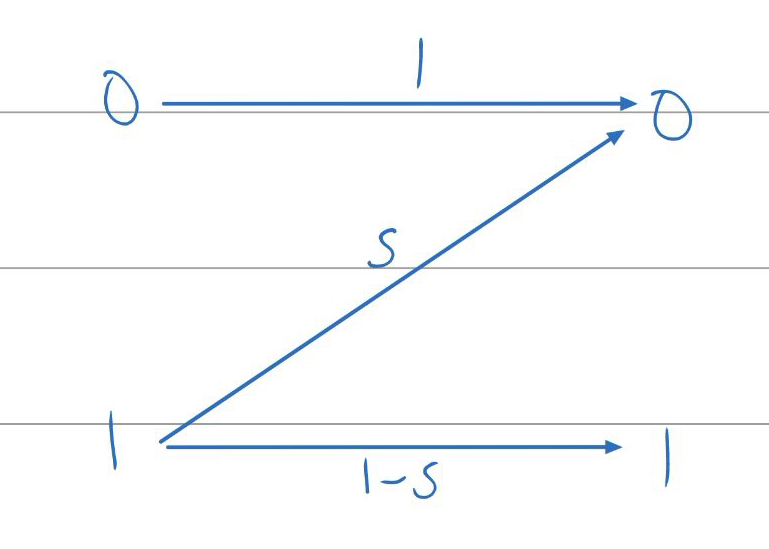
\includegraphics[scale=0.2]{1}
            \label{fig:figure1}
            \end{figure}
        \subitem(b)
            \begin{figure}[htbp]
            \centering
            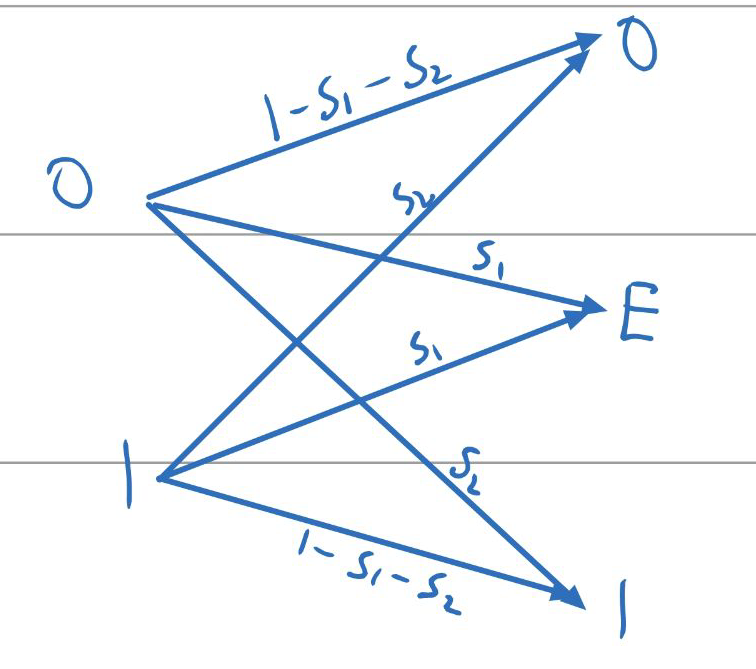
\includegraphics[scale=0.2]{2}
            \label{fig:figure2}
            \end{figure}
        \subitem(c)
            \begin{figure}[htbp]
            \centering
            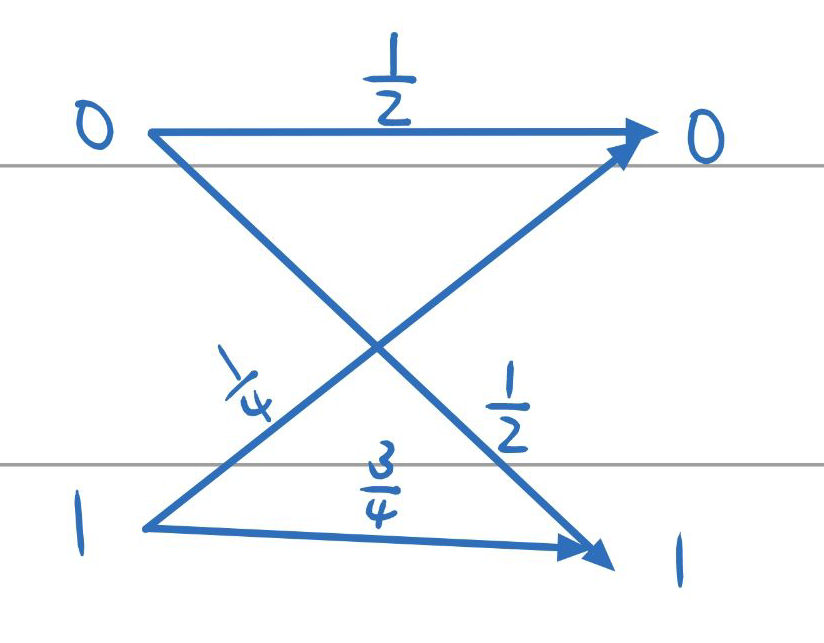
\includegraphics[scale=0.2]{3}
            \label{fig:figure3}
            \end{figure}
        \subitem(d)
            \begin{figure}[htbp]
            \centering
            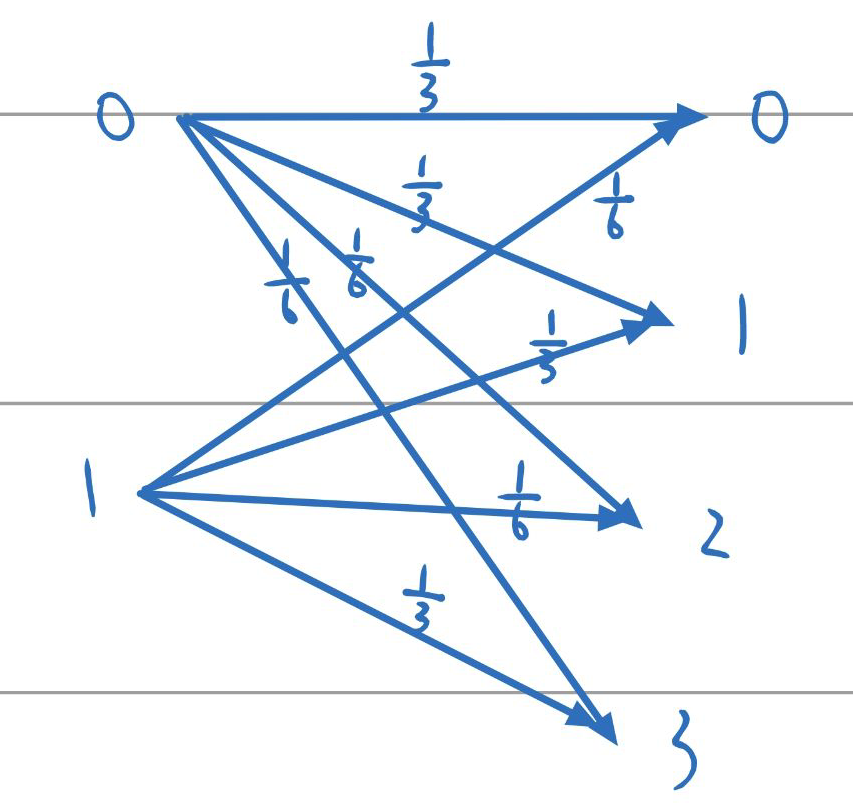
\includegraphics[scale=0.2]{4}
            \label{fig:figure4}
            \end{figure}
\\
\\
\\
    \item[Problem 2] Solutions:
    \subsection*{Channel Model}
Given the channel is memoryless and the noise \(Z\) is additive and independent of the input \(X\), the output \(Y\) can be expressed as:
\[
Y = X \oplus Z
\]
where \(\oplus\) denotes the binary addition (XOR).

\subsection*{Channel Matrix}
The channel transition probabilities are:
\[
\begin{array}{|c|c|c|}
\hline
X \backslash Y & 0 & 1 \\
\hline
0 & \Pr[Z=0] & \Pr[Z=a] \\
1 & \Pr[Z=a] & \Pr[Z=0] \\
\hline
\end{array}
\]
with \(\Pr[Z = 0] = \Pr[Z = a] = \frac{1}{2}\).

\subsection*{Channel Capacity Calculation}
The channel capacity \(C\) is given by:
\[
C = \max_{p(x)} I(X; Y)
\]
Using the symmetry of the channel and the uniform distribution of \(Z\), the mutual information \(I(X; Y)\) is maximized when \(X\) is also uniformly distributed. This gives us:
\[
I(X; Y) = H(Y) - H(Y|X)
\]
Since \(Y = X \oplus Z\), and both \(X\) and \(Z\) are independent and uniformly distributed:
\[
H(Y) = 1 \text{ bit (Entropy of a fair coin)}
\]
\[
H(Y|X) = H(Z) = 1 \text{ bit}
\]
\[
C = 1 - 1 = 0 \text{ bits}
\]
This indicates that the capacity of this channel is 0 bits per channel use, meaning no reliable communication is possible if \(a = 0\). If \(a \neq 0\), further analysis on the value of \(a\) would be required to compute its specific impact on the channel capacity.

    \item[Problem 3] Solutions:
        \subitem(a)
            Given the transition probabilities shown in the figure:
                \[
                \begin{array}{|c|c|c|c|}
                \hline
                X \backslash Y & 0 & E & 1 \\
                \hline
                0 & 1 - \alpha - e & \alpha & e \\
                1 & e & \alpha & 1 - \alpha - e \\
                \hline
                \end{array}
                \]

                The capacity \(C\) of this channel is given by:
                \[
                C = \max_{p(x)} I(X; Y)
                \]
                where \(I(X; Y)\) is the mutual information between \(X\) and \(Y\). Assume \(X\) is distributed Bernoulli(0.5) for symmetry. The capacity can then be computed as:
                \[
                C = 1 - H_b(e) - \alpha \log(2)
                \]
                where \(H_b(p)\) is the binary entropy function \( -p \log_2(p) - (1-p) \log_2(1-p) \).
        \subitem(b)
            \[C = 1 - H_b(e)\]
        \subitem(c)
            \[C = 1 - \alpha\]


\end{description}


\end{document}
